% ============================================================
% LLM-BLM 実験 11：決算発表文の読ませ方とまとめ方の修正 1〜5、開発と最後の比較
% コンパイル：tectonic -X compile LLM-BLM_実験11.tex   （XeTeX 系。このフォルダで実行する）
% 図は 図/（作成スクリプト/figs.py が experiments/F_fixes/results から作る）
% 数値の出どころは experiments/F_fixes/results の JSON と findings.md、事前登録は experiments/F_fixes/preregistration.md
% ============================================================
\documentclass[xelatex,ja=standard,jafont=haranoaji,a4paper,10pt,openany]{bxjsreport}
\setpagelayout*{left=24mm,right=24mm,top=24mm,bottom=26mm,footskip=11mm}

\usepackage{amsmath,amssymb,mathtools,bm}
\usepackage{booktabs,array,multirow,longtable}
\usepackage{graphicx}
\usepackage{adjustbox}
\usepackage{xcolor}
\usepackage{tikz}
\usetikzlibrary{arrows.meta,positioning,calc,fit}
\usepackage{enumitem}
\usepackage{caption}
\usepackage{float}
\usepackage[most]{tcolorbox}
\usepackage[hidelinks,bookmarksnumbered]{hyperref}
\pdfstringdefDisableCommands{\def\Omega{Ω}\def\tau{τ}\def\Sigma{Σ}}

\graphicspath{{図/}}

\definecolor{c1}{HTML}{2A78D6}
\definecolor{c2}{HTML}{EB6834}
\definecolor{c3}{HTML}{1BAF7A}
\definecolor{c4}{HTML}{EDA100}
\definecolor{c7}{HTML}{6250D6}
\definecolor{ink2}{HTML}{52514E}
\definecolor{soft1}{HTML}{E4EEF9}
\definecolor{soft2}{HTML}{FBEEDF}
\definecolor{soft3}{HTML}{E3F3E9}
\definecolor{soft4}{HTML}{EEE8FA}
\definecolor{soft5}{HTML}{FDF3DA}

\newcommand{\code}[1]{\texttt{#1}}
\newcommand{\SP}{S\&P500}
\newcommand{\figref}[1]{図~\ref{#1}}
\newcommand{\tabref}[1]{表~\ref{#1}}
\newcommand{\chapref}[1]{第~\ref{#1}~章}
\newcommand{\secref}[1]{\ref{#1}~節}

\setlist[itemize]{leftmargin=1.6em,itemsep=0.2em,topsep=0.4em}
\setlist[enumerate]{leftmargin=1.8em,itemsep=0.2em,topsep=0.4em}
\captionsetup{font=small,labelfont=bf,skip=6pt}
\renewcommand{\arraystretch}{1.2}
\setlength{\LTpre}{6pt}
\setlength{\LTpost}{6pt}

\makeatletter
\def\@makechapterhead#1{\vspace*{0.3\Cvs}{\parindent\z@\raggedright\normalfont
  \ifnum\c@secnumdepth>\m@ne\if@mainmatter{\Large\headfont\@chapapp\thechapter\@chappos}\par\nobreak\vskip0.4\Cvs\fi\fi
  \interlinepenalty\@M\LARGE\headfont #1\par\nobreak\vskip 1.5\Cvs}}
\def\@makeschapterhead#1{\vspace*{0.3\Cvs}{\parindent\z@\raggedright\normalfont
  \interlinepenalty\@M\LARGE\headfont #1\par\nobreak\vskip 1.5\Cvs}}
\makeatother

\newtcolorbox{keybox}[1][要点]{enhanced,breakable,colback=soft1,colframe=c1,boxrule=0.5pt,arc=2pt,
  left=8pt,right=8pt,top=6pt,bottom=6pt,title={#1},fonttitle=\sffamily\bfseries\small,coltitle=white}
\newtcolorbox{notebox}[1][注意]{enhanced,breakable,colback=soft2,colframe=c2,boxrule=0.5pt,arc=2pt,
  left=8pt,right=8pt,top=6pt,bottom=6pt,title={#1},fonttitle=\sffamily\bfseries\small,coltitle=white}
\newtcolorbox{verdict}[1][判定]{enhanced,breakable,colback=soft4,colframe=c7,boxrule=0.5pt,arc=2pt,
  left=8pt,right=8pt,top=6pt,bottom=6pt,title={#1},fonttitle=\sffamily\bfseries\small,coltitle=white}

\tikzset{
  box/.style={draw=#1,fill=#1!8,rounded corners=2pt,align=center,font=\footnotesize,inner sep=4pt,
              minimum height=10mm,text width=24mm},
  arr/.style={-{Stealth[length=2mm]},color=ink2,line width=0.6pt},
}

\title{LLM-BLM 実験 11\\[6pt]
  \large 決算発表文の読ませ方とまとめ方の修正：\\先読みのない LLM は、小技なしでも NLP を超えるか}
\author{実験の結果の報告書}
\date{2026 年 10 月 21 日}

\begin{document}
\maketitle

% ============================================================
\chapter*{概要}
\addcontentsline{toc}{chapter}{概要}

LLM や NLP が決算発表文を読むとき、読める長さは限られている（ChronoGPT は約 7,000 字、gpt-4o-mini は先頭 15,000 字）。発表文の後半は、ばらけた表や免責事項が多い。そこで、文献調査で挙がった「少ない読む量で効果を上げる」修正 5 つを試した。

\begin{itemize}
\item 修正 1：表の切れ端と定型文を除く
\item 修正 2：FinBERT の読む範囲を変える（先頭＋末尾、全文）
\item 修正 3：会社ごとの点数をセクターにまとめる方法
\item 修正 4：ChronoGPT の埋め込みの取り方（真ん中の層、最後のトークン）
\item 修正 5：LLMLingua-2 で文章を圧縮する
\end{itemize}

開発用のモデル（先読みのない ChronoGPT と NLP）で修正を試し、残すかどうかは人ではなく事前に決めた規則が決めた。そのあと、まだ使っていない最終の期間で、gpt-4o-mini・ロジスティック回帰・反応で追加学習した BERT と並べて、1 回だけ比べた。

\begin{keybox}[主な結論]
\begin{itemize}
\item \textbf{修正はほとんど残らなかった。}表の切れ端や定型文を除いても、反応の説明力はほぼ変わらない（大事な記述はもともと先頭にある）。まとめ方も、今のやり方（直近の発表、時価総額加重）が最良だった。
\item \textbf{それでも、先読みのない ChronoGPT は NLP を超えた（主な検定は支持）。}2020 年以降の 13,141 本で、数字の統制と辞書・FinBERT・TF-IDF を超えて、1 標準偏差あたり $+34$bp（$t$ 4.8、置換の $p=0.001$）。期間の切り方を変えた 3 通りすべてで支持。
\item \textbf{探索：効いたのは埋め込みの取り方だった。}ChronoGPT の真ん中の層を使うと、開発の期間の説明力が約 1.6 倍になった（3 通りすべてで差の $t$ 2 以上）。ただし、規則の順番のせいで本番の判定には入っていない。圧縮（修正 5）ははっきり悪くなった。
\item \textbf{セクター単位の BLM では、どのモデルも効かなかった。}
\end{itemize}
\end{keybox}

\setcounter{tocdepth}{1}
{\small\tableofcontents}

% ============================================================
\chapter{目的と設計}\label{ch:design}

\section{問い}

\begin{verdict}[問い]
\textbf{主}：修正後の先読みのない ChronoGPT は、数字の統制と、修正後の NLP 3 つ（辞書・FinBERT・TF-IDF）を超えて、決算発表への 2 取引日の反応を説明するか。\\
\textbf{副}：修正 1〜5 は、それぞれのモデルの説明力を上げるか。修正後のモデルは、gpt-4o-mini・ロジスティック回帰・反応で追加学習した BERT と並べるとどうか。セクター単位の BLM ではどうか。
\end{verdict}

\section{期間の分け方}

修正を何度も試した期間で最終の比較をすると、良く見える修正を選んだ分だけ結果が甘くなる。期間を開発と最終に分け、切り方を 3 通り用意した。

\begin{table}[H]
\centering
\caption{期間の切り方。主な結果は B。A と C は確認用。}
\small
\begin{tabular}{llll}
\toprule
切り方 & 開発 & 最終 & 最終の月数 \\
\midrule
\textbf{B（主）} & 2016〜2019 年 & 2020-01〜2026-08 & 約 80 か月 \\
A & 2016〜2020 年 & 2021-01〜2026-08 & 約 68 か月 \\
C & 2016〜2022 年 & 2023-01〜2026-08 & 約 44 か月 \\
\bottomrule
\end{tabular}
\end{table}

C の開発の期間は A・B の最終の期間に重なる。そこで、修正を残すかどうかは人が選ばず、事前にコードで固定した規則が切り方ごとに機械的に決めた。

\section{残すかどうかの規則}

\begin{enumerate}
\item 修正前と比べて主な指標が良くなり、その差の $t$ が 1 以上（会社ごと：同じ発表どうしで当てはまりの差を比べ、発表日ごとにまとめた標準誤差。セクターごと：月ごとの IC の差の Newey--West の $t$）。
\item 開発の期間の前半と後半のどちらでも悪くならない。
\item 順番：修正 1 → （修正 1 が残れば）修正 2・4・5 → 修正 3。
\end{enumerate}

\section{モデルと比べる相手}

\begin{itemize}
\item \textbf{ChronoGPT}：全期間で版 2015（2015 年末までの文章で学習）に揃えた。2016 年以降には先読みがない。埋め込みの上に、四半期ごとに過去の発表だけで学習するリッジ回帰を置く（実験 5 と同じ）。
\item \textbf{NLP}：辞書（Loughran--McDonald）、FinBERT（学習なし）、TF-IDF＋リッジ（四半期ごとに学び直す）。
\item \textbf{ロジスティック回帰}：数字の説明変数だけで、反応の符号を当てる。
\item \textbf{BERT（追加学習）}：実験 4 の FinBERT の追加学習を、切り方ごとに開発の終わりまでの反応で学び直したもの。
\item \textbf{gpt-4o-mini}：最後の比較だけに使う（開発では一度も使わない）。期間は 2023-11 以降。
\end{itemize}

TF-IDF は新しい言葉を覚え直し、FinBERT は 2019 年までの文章を知っている。ChronoGPT には不利な条件での比較である。

% ============================================================
\chapter{実行の記録}\label{ch:record}

事前登録とコードを固定してから、点数付け・開発の判定・最後の比較をそれぞれ 1 回だけ行った。途中で起きたことを、すべて記録する。

\begin{notebox}[事前登録の後に直したこと（どれも、どの点数の評価よりも前）]
\begin{itemize}
\item \textbf{修正 5 を行った。}事前に決めた確認で、修正 1 の後でも見通しの語が ChronoGPT の読む範囲の外にある発表が 10.7\%（基準 10\% 以上）だったため。圧縮用のモデル（LLMLingua-2、MIT）とそのコードを、評価の前に追加した。
\item \textbf{修正 1 の規則の穴を直した。}最初の規則は、定型文の語やメールアドレスを 1 つでも含む行を、行ごと捨てていた。要約がまるごと 1 行に詰まった発表では、大事な中身まで消えていた（1,500 本の抜き出しで約 15\%）。開発の判定が別の理由（文章が空になる発表）で止まったときに見つけ、文単位で定型文だけを捨てる形に直して、点数を作り直した。直した後の確認で、消える「見通し」の語は、見出しだけの行・免責事項・説明会の案内の中のものだけだった。
\item 直した後も文章が何も残らない 14 本（本文が見出しだけの発表）は、その修正の点数を「なし」として比較から除いた。
\end{itemize}
\end{notebox}

\begin{itemize}
\item 計算はすべてこの PC（RTX 5050）で行った（約 19 時間）。一度、借りた GPU（RunPod、RTX 4090）で回したが、結果をダウンロードする前に止めてしまい、消えたので使っていない。
\item 修正 1 で除いた文字は平均 27\%。
\item 規則の判定で切り方 B では修正 1 が残らなかったので、事前に決めた条件どおり、gpt-4o-mini の付け直しは行わなかった（費用 0 円）。
\end{itemize}

% ============================================================
\chapter{開発の結果}\label{ch:dev}

\section{修正 1 は、ほとんど差がなかった}

\begin{figure}[H]
\centering
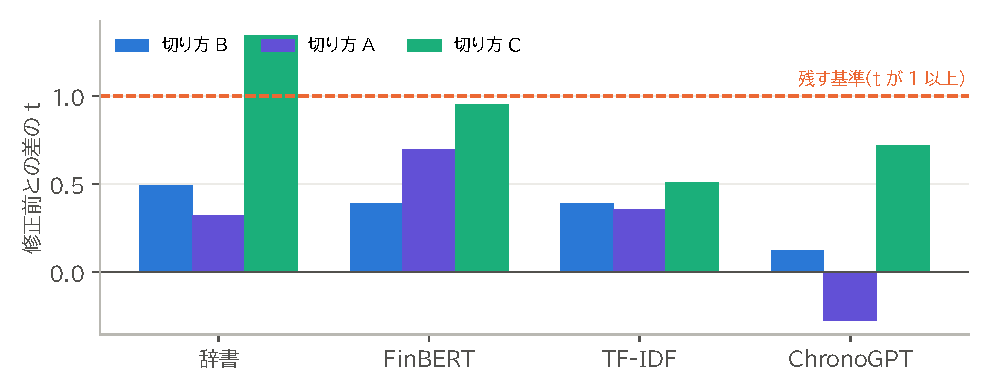
\includegraphics[width=0.85\linewidth]{dev_fix1.pdf}
\caption{開発の期間での、修正 1（表の切れ端と定型文を除く）と修正前の差の $t$。破線が残す基準。}
\label{fig:dev1}
\end{figure}

\begin{table}[H]
\centering
\caption{開発の判定で残った修正。}
\small
\begin{tabular}{lll}
\toprule
切り方 & 残った修正 & まとめ方 \\
\midrule
B（主） & なし & 今のまま（直近 92 日、時価総額加重） \\
A & なし & 今のまま \\
C & 辞書の修正 1 だけ（差の $t$ 1.34） & 今のまま \\
\bottomrule
\end{tabular}
\end{table}

\begin{itemize}
\item 修正 1 の差は、どのモデルでも決定係数で $\pm 0.0005$ ポイント以内と、ほぼ 0 だった（\figref{fig:dev1}）。大事な記述（要約と見通し）は、もともと発表の先頭にある。
\item 修正 3（まとめ方）：直近の発表を日数で弱める形も、単純平均も、今のやり方を超えなかった。単純平均は、どのモデル・切り方でも悪くなった（差の $t$ はおおむね $-1$〜$-3$）。セクターの見通しは、セクターの値動きを決める大きな会社の読み取りで作るほうがよい。
\item 修正 2・4・5 は、順番の規則（修正 1 が残ったときだけ試す）により、FinBERT と ChronoGPT では判定に進まなかった。
\end{itemize}

\section{探索：試されなかった修正 2・4・5}

順番の規則で判定に進まなかった修正を、事前登録とは別の探索として、修正前と直接比べた。

\begin{figure}[H]
\centering
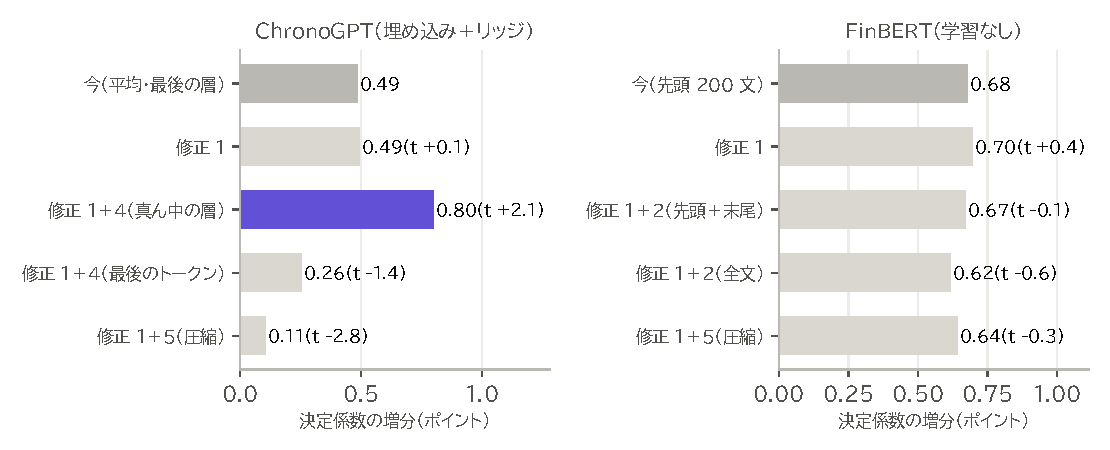
\includegraphics[width=0.98\linewidth]{explore_245.pdf}
\caption{切り方 B の開発の期間で、数字の統制に加えたときの決定係数の増分。括弧は修正前との差の $t$。色の濃い棒が、規則の基準を満たすもの。探索の結果で、判定には使っていない。}
\label{fig:explore}
\end{figure}

\begin{itemize}
\item \textbf{ChronoGPT の真ん中の層（修正 4）が、はっきり良かった。}増分は 0.49 → 0.80 ポイント（約 1.6 倍）。3 つの切り方すべてで差の $t$ が 2 以上（B 2.07、A 2.57、C 2.86）で、規則で試されていれば残っていた（\figref{fig:explore}）。最後の層は次の単語を当てることに特化していて、真ん中の層のほうが文章の意味をよく持っている、という文献の指摘と合う。
\item 最後のトークンは悪くなった（$t$ $-1.4$〜$-2.0$）。
\item \textbf{圧縮（修正 5）は、はっきり悪くなった}（ChronoGPT で $t$ $-2.8$〜$-4.3$）。単語を間引いた崩れた文章を、ChronoGPT はうまく読めない。
\item FinBERT の読む範囲の変更（修正 2）と圧縮は、どれも良くならなかった。
\end{itemize}

% ============================================================
\chapter{最後の比較}\label{ch:final}

\section{主な検定}

\begin{verdict}
\textbf{支持。}切り方 B の最終の期間（2020-01〜2026-08、13,141 本）で、ChronoGPT の係数は 1 標準偏差あたり $+34.3$bp（95\% 区間 $+20.3$〜$+48.4$、$t=4.79$）、置換の片側 $p=0.001$。統制は、数字の説明変数と、辞書・FinBERT・TF-IDF。
\end{verdict}

\begin{table}[H]
\centering
\caption{主な検定（修正が残らなかったので、ChronoGPT と NLP は修正前と同じ）。}
\small
\begin{tabular}{lrrrrl}
\toprule
切り方 & 本数 & 係数（bp） & $t$ & 置換の $p$ & 判定 \\
\midrule
\textbf{B（主）} & 13,141 & $+34.3$ & 4.79 & 0.001 & 支持 \\
A & 11,252 & $+38.1$ & 4.88 & 0.001 & 支持 \\
C & 7,448 & $+37.0$ & 3.51 & 0.001 & 支持 \\
gpt-4o-mini の期間（参考） & 5,706 & $+47.8$ & 3.79 & — & — \\
\bottomrule
\end{tabular}
\end{table}

\section{会社ごとの比較}

\begin{figure}[H]
\centering
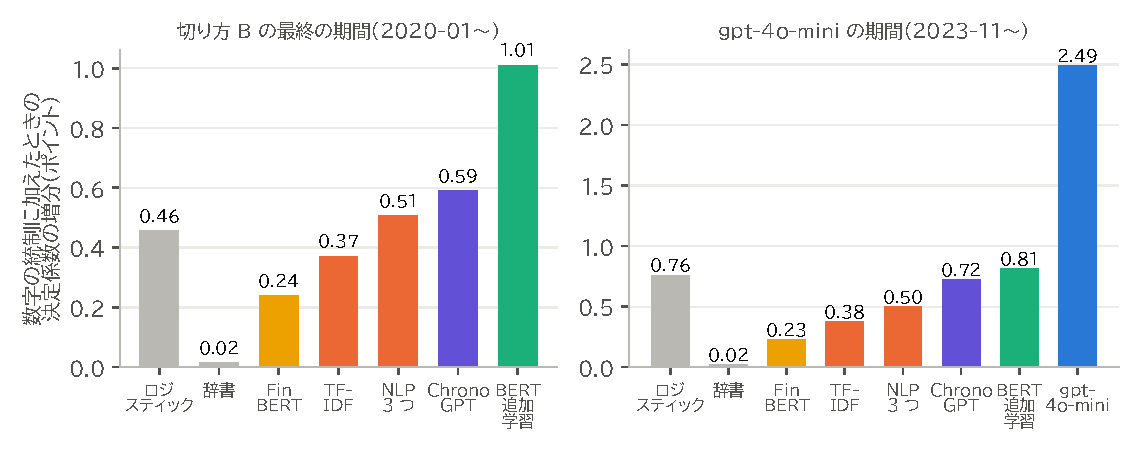
\includegraphics[width=0.98\linewidth]{final_firm.pdf}
\caption{数字の統制に、それぞれを 1 つずつ加えたときの決定係数の増分。左：切り方 B の最終の期間。右：gpt-4o-mini の点数がある期間。}
\label{fig:firm}
\end{figure}

\begin{itemize}
\item ChronoGPT（$+0.59$ ポイント）は、NLP 3 つをまとめたもの（$+0.51$）より大きい。
\item 反応で学習した BERT（$+1.01$）は ChronoGPT より大きい。学習なしの gpt-4o-mini は、短い期間で $+2.49$ と群を抜く（同じ期間で ChronoGPT は $+0.72$）。実験 4・5 と同じ並び。
\end{itemize}

\begin{notebox}[ロジスティック回帰の作りの弱さ（探索で確かめた）]
事前登録したロジスティック回帰は、外れ値に弱かった。アナリスト予想との差には $-500\%$ のような極端な値があり、標準化するとふつうの値が押しつぶされる。そのため、全体の予測の当たり具合（AUC 0.593）が、アナリスト予想との差 1 つだけ（0.612）より低くなり、文章の点数を足すと AUC がむしろ下がった。変数を学習期間の中での順位に直すと（探索）、土台の AUC は 0.611 になり、ChronoGPT を足すと $+0.0026$（95\% 区間 $+0.0005$〜$+0.0047$）上がった。AUC の比較は、この版で読むのがよい。
\end{notebox}

\section{セクター単位}

\begin{figure}[H]
\centering
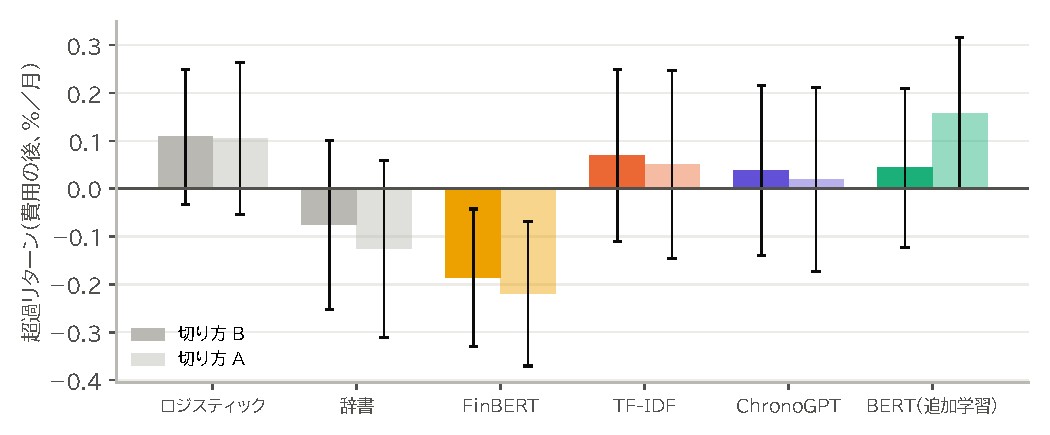
\includegraphics[width=0.92\linewidth]{final_sector.pdf}
\caption{セクター単位の BLM（11 セクター＋米国債、TE の上限 3\%、片道 0.1\% の費用）の、時価総額に対する月次の超過リターン（95\% 区間）。濃い色が切り方 B、薄い色が A。}
\label{fig:sector}
\end{figure}

どのモデルも、費用の後で有意に時価総額を上回らなかった（\figref{fig:sector}）。翌月のセクターのリターンとの順位相関（IC）も、ロジスティック回帰（$+0.08$、$t$ 2.6）以外はほぼ 0 だった。学習なしの FinBERT は月 $-0.19\%$（$t$ $-2.5$）と悪かった。決算発表の情報は月次の見通しにはほとんど残らない、という実験 7〜9 の結論と同じである。

% ============================================================
\chapter{考察と限界}\label{ch:discussion}

\section{何が分かったか}

\begin{enumerate}
\item \textbf{読ませ方の小技（不要な部分を除く、範囲を変える、圧縮する）は、ほとんど効かない。}決算発表の大事な記述は先頭にまとまっていて、今の読み方でも読めていた。圧縮はむしろ害になる。
\item \textbf{効く可能性があるのは、モデルの中のどこを取り出すか（真ん中の層）。}ただし探索の結果で、確かめるには新しい事前登録が要る。最終の期間はもう見たので、新しい確認では、まだ使っていない評価（たとえば翌年の発表）を用意する必要がある。
\item \textbf{先読みのない LLM は、小技なしでも NLP を超える情報を持つ。}5 年以上の期間で、3 通りの切り方すべてで支持された。
\item \textbf{それでも、反応で学習した BERT と、大きな LLM（gpt-4o-mini）には及ばない。}
\end{enumerate}

\section{限界}

\begin{itemize}
\item 修正 1 の規則に穴があり、点数の評価の前に直した。
\item 順番の規則のせいで、修正 2・4・5 は本番の判定に進まなかった。修正 1 の成否と、ほかの修正の成否を結び付けたのは設計の誤りだった。
\item 事前登録したロジスティック回帰は外れ値に弱かった（順位の版は探索）。
\item 開発の期間（2016〜2019 年）は、実験 2〜5 で反応を一度見た期間。
\item gpt-4o-mini の期間は約 33 か月と短い。
\end{itemize}

% ============================================================
\chapter*{再現の手順}
\addcontentsline{toc}{chapter}{再現の手順}

\begin{verbatim}
python experiments/F_fixes/score.py stats dictionary finbert chrono_raw chrono
python experiments/F_fixes/score.py compress finbert5 chrono5
python experiments/F_fixes/develop.py      # 開発の判定（規則で機械的に）
python experiments/F_fixes/bert.py         # BERT の学び直し（切り方ごと）
python experiments/F_fixes/gpt.py          # 条件つき（今回は行わず）
python experiments/F_fixes/final.py        # 最後の比較（1 回だけ）
python experiments/F_fixes/explore_fixes245.py     # 探索
python experiments/F_fixes/explore_rank_logit.py   # 探索
\end{verbatim}

数値の出どころは \code{experiments/F\_fixes/results/} の JSON と \code{findings.md}、事前登録は \code{experiments/F\_fixes/preregistration.md}。費用はこの PC の分は 0 円（RunPod で回して結果が消えた分に、数ドルかかった）。

\end{document}
